\section{Durchführung}
\label{sec:Durchführung}

Um den Eingang kosmischer Myonen zuverlässig mit einem Szinitllatortank messen zu können ist es besonders wichtig mögliche Störsignale herauszufiltern. Wie dies genauer funktioniert, wird in folgendem Unterkapitel besprochen.

\subsection{Versuchsaufbau}


Die Detektion der Myonensignale erfolgt in einem rund $\qty{50}{\liter}$ großen zylinderförmigen Szinitllatortank. Hier wird ein organischer Szintillator verwendet, da so die für die Bestimmung der Lebenszeit wichtige Zeitauflösung erhöht wird. An beiden Seiten des Szintillatortanks befinden sich Photomultiplier (PMTs), die von einer Hochspannungsquelle betrieben werden. Diese verstärken dann alle Signale die im Szintillator eingehen. \\

Um nun aus den von den PMTs ausgehendenden Signalen nur Signale von Myonen, die im Szinitllatortank zerfallen herauszufiltern, werden die PMT-Signale in einer Koinzidenzschaltung zusammengeführt. 
Dazu werden die PMT-Signale zuerst jeweils über eine Verzögerungsleitung in einen Diskriminator mit variabler Schwelle geführt, dessen Ausgangsimpulslänge ebenfalls eingestellt werden kann. Diese beiden Signale werden dann in einer Koinzidenz zusammengeführen, welche dann im besten Fall nur ein Signal liefert, wenn an den PMTs gleichzeitig ein Signal eingeht um so die Dunkelrate durch thermische Elektronen im Material zu minimieren.\\

Um nun die exponentiell verteilte Zerfallszeit der Myonen im Material zu messen, wird das Ausgangssignal der Koinzidenz, wie in \autoref{fig:aufbau} genauer zu sehen, über zwei UND-Gatter und einem Monoflop an das Startsignal eines Time-Amplitude-Converters (TAC) gesendet.


An dem Monoflop kann außerdem eine Suchzeit $T_S$ eingestellt werden innerhalb der nach einem weiteren Eingangssignal gesucht wird. Tritt dieser Fall ein, geht also innerhalb der Suchzeit ein weiteres Signal ein, hat dies die Signatur eines Myons das im Szintillator gestoppt hat, dort nach einer zufälligen Zeit $t$ zerfallen ist und ein Elektron ausgesendet hat. Da allerdings nicht zwischen dem Zerfall eines gestoppten Myons und dem Eingang eines weiteren Myons unterschieden werden kann, darf hier die Suchzeit nicht zu groß sein. Das innerhalb der Suchzeit gemessene Eingangssignal löst dann ein Stoppsignal am TAC aus. Um hier zu verhindern, dass das Startsignal auch direkt als Stoppsignal gemessen wird, ist hier eine weitere Verzögerungsleitung von $\Delta t = \qty{30}{\nano\second}$ zwischen Koinzidenz und Monoflop eingebaut. Die gemessene Zeit am TAC wird dann an einen Multichannelanalysator (MCA) übergeben, der die gemessene Zeit histogrammatisch in verschiedene Channel unterteilt und diese dann am PC ausgelesen werden können.
Die Start- und Stopsignale am TAC werden außerdem mit einem Impulszäler zur Überprüfung der Zählraten verbunden. \\



Der Gesamtaufbau des Versuchs wird übersichtshalber zusätzlich in \autoref{fig:aufbau} als Blockschaltbild dargestellt. \\

\begin{figure}[htbp]
    \centering
    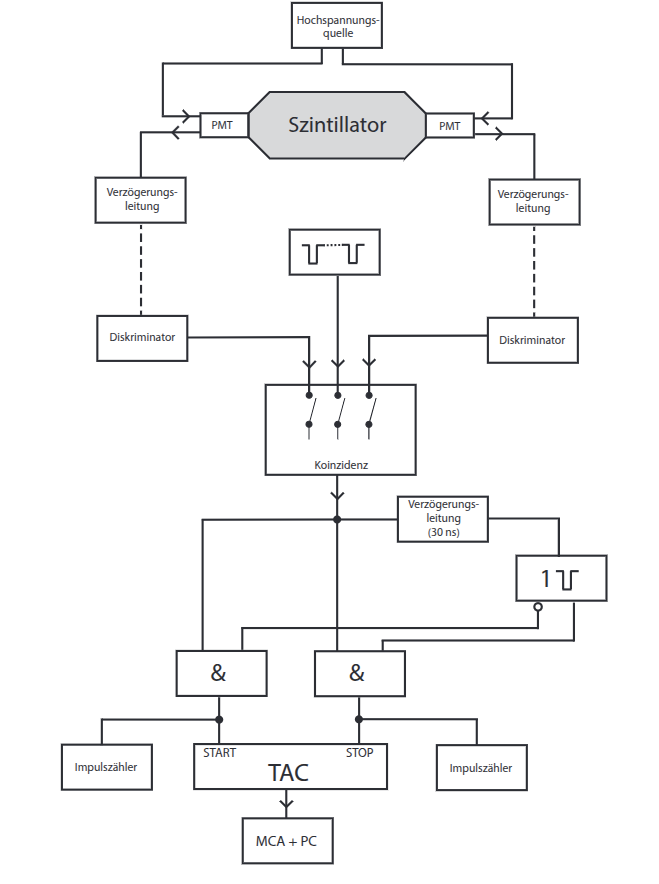
\includegraphics[width=0.7\textwidth]{content/pics/aufbau.png}
    \caption{Versuchsaufbau als Blockschaltbild~\cite{Durchfuhrung}.}
    \label{fig:aufbau}
\end{figure}


\vspace{1cm}

\subsection{Versuchsdurchführung}
\begin{enumerate}
    \item \textbf{Einstellung der Diskriminatoren} \\
    Zuerst wird die Spannung an den PMTs jeweils in einem Bereich von ca. $\qty{1600}{\volt}$ - $\qty{1900}{\volt}$ eingestellt. 
    Dann wird an beiden Diskriminatoren die Schwelle so eingestellt, dass die Impulsrate an beiden Ausgängen bei ca. $30 \, \mathrm{Hz}$ liegt. Diese kann mithilfe der Impulszähler überprüft werden. Außserdem wird die Ausgangsimpulsdauer beider Diskriminatoren auf einen Bereich von $10-\qty{20}{\nano\second}$ mithilfe eines Oszilloskops eingestellt.
    \item \textbf{Einstellung der Verzögerungsleitung und Koinzidenz} \\
    Im nächsten Schritt wird nun die Impulsrate an der Koinzidenz für verschiedene Verzögerungszeiten jeweils an beiden Verzögerungsleitungen zwischen den Diskriminatoren und PMTs gemessen und aufgeschrieben. Es werden soviele Messwerte genommen, dass die Halbwertsbreite der Verteilung bestimmbar ist. Anhand dieser Werte wird dann eine geeignete Verzögerung mit möglichst großer Impulsrate ausgewählt, sodass möglichst eine Impulsrate von $\qty{20}{\hertz}$ an der Konizidenz übrig bleibt.
    \item \textbf{Kalibrierung des MCAs} \\
    Um die Channelnummer des MCAs in eine Messzeit übersetzen zu können, wird nun das MCA mittels eines Doppelimpulsgenerators kalibriert. Dazu wird der Doppelimpulsgenerator an den MCA angeschlossen, welcher dann Doppelimpulse mit einer variabel einstellbaren Verzögerung erzeugt. Die Verzögerung wird hier in einem Bereich von $\qty{0.5}{\micro \second}$ - $\qty{9.9}{\micro\second}$ in $\qty{0.5}{\micro \second}$-Schritten variiert und die korresponiderende Channelnummer am MCA notiert. 
    \item \textbf{Messung der kosmischen Myonen} \\
    Zuletzt wird nun die Koinzidenz mit dem TAC gemäß dem in \autoref {fig:aufbau} zu sehenden Schaltbild verkabelt und am Monoflop eine Suchzeit eingestellt. Der TAC wird mit dem MCA verbunden und die Messung kann gestartet werden. 

\end{enumerate}
\clearpage